% mycsrf 'for beeing included' snippet template
%
% (c) Karsten Reincke, Frankfurt a.M. 2012, ff.
%
% This text is licensed under the Creative Commons Attribution 3.0 Germany
% License (http://creativecommons.org/licenses/by/3.0/de/): Feel free to share
% (to copy, distribute and transmit) or to remix (to adapt) it, if you respect
% how you must attribute the work in the manner specified by the author(s):
% \newline
% In an internet based reuse please link the reused parts to mycsrf.fodina.de
% and mention the original author Karsten Reincke in a suitable manner. In a
% paper-like reuse please insert a short hint to mycsrf.fodina.de and to the
% original author, Karsten Reincke, into your preface. For normal quotations
% please use the scientific standard to cite
%


%% use all entries of the bibliography

\section{Anliegen}

Es gibt 'zweieinhalb' Dinge, die man erreichen möchte, wenn man am Computer
Notentexte 'schreibt':

\begin{itemize}
  \item Zum ersten wird man seine Werke hörbar machen wollen, also in
  Computersound umwandeln. Dies ist -- bis auf eine Ausnahme -- nicht
  unser Thema.
  \item Zum zweiten wird man seine Noten ausdrucken wollen, möglichst
  ansprechend und so leserlich, dass spielbare Notenblätter für Musiker
  entstehen. Dies werden wir allenfalls implizit behandeln.
  \item Und schließlich wird der eine oder andere Autor Notenbeispiele in seine
  (musikwissenschaftlichen) Texte einbinden wollen. Wie man das in welchen
  Grenzen mit \LaTeX\ umsetzt, wollen wir hier diskutieren und demonstrieren.
\end{itemize}

Natürlich ist die Integration von Noten in wissenschaftliche Texte nicht ein
grundsätzlich anderes Szenario als der bloße Druck eines Notenblattes.
Denn auch eine am Computer erstellte musikwissenschaftliche Arbeit zielt zuletzt
auf eine ansprechende Erscheinung. Gleichwohl fordert sie Besonderes: Anders als
ein Notenblatt enthält sie vornehmlich Fließtext. Außerdem nutzt sie
üblicherweise keine ganzen Werke als Beleg, sondern Ausschnitte. Zu guter Letzt
fordert die Musikwissenschaft gelegentlich, in diese 'Extrakte' Zeichen oder
Kommentare einfügen zu können, die selbst nicht zur 'Notensprache'
gehören.\footnote{Ein Beispiel dafür ist die 'Harmonieanalyse', die ja eine
eigene Fachsprache bereitstellt und erwartet, dass z.B. die Abkürzungen für
\textit{Tonika}, \textit{Subdominante} oder \textit{Dominante} samt
Subspezifikatoren in den entsprechenden Notentext eingebunden werden.}

Die beste Methode, wissenschaftliche Texte zu schreiben, bietet \LaTeX\ --
ebenso gemessen am Druckbild, wie am Grad der Automatisierung oder am Aufwand,
den (ei\-ge\-nen) Wissenschaftsvorgaben konsistent gerecht zu werden. Und so
geht es hier -- vereinfacht gesagt -- um \LaTeX\ und Musik. Ein Blick auf
CTAN-Liste mit entsprechenden Tools\footnote{$\rightarrow$
\lnkb{https://ctan.org/topic/music}{2018-12-27}} verwirrt eher, als dass er
hilft: Womit soll man anfangen, was braucht man wozu, was davon soll man lernen,
was lohnt überhaupt die Mühe? Google beantwortet die Query
$\langle$\textit{latex music}$\rangle$\footnote{$\rightarrow$
\lnka{https://www.google.com/search?q=latex+music}} mit Links auf einige kurze
Artikel und auf die bekannten Tools \textit{MusiX\TeX} und \textit{LilyPond}.
Zusammen führt auch das den unbedarften Anfänger nicht weiter. Es fehlt einfach
eine qualifizierte Sichtung und Anleitung, die sagt und zeigt, wie man das beste
Ergebnis mit geringstem Aufwand erreicht. Diese Lücke wollen wir mit einem
selbstreferentiellen Dokument schließen: Es sichtet, was es gibt, zeigt, wie
geht, und beleuchtet, was warum nicht funktioniert. Dabei soll alles, was es
vorgeführt, anhand des eigenen \LaTeX-Quelltexts reproduzierbar sein. Und wenn
es uns damit gelingt, den einen oder anderen davon abgehalten zu haben, auf's
falsche Pferd zu setzen, dann wollen wir zufrieden sein.

Den wissenschaftlichen Text unseres 'Demos' erzeugen wir mit
\textit{mycsrf}\footcite[vgl.][\nopage wp.]{Reincke2018a}, einem Bibliographie-
und Zitierstil\footnote{Genau genommen handelt es sich dabei nicht um einen
eigenständigen Zitierstil, der in das \LaTeX-System zu installieren wäre,
sondern um eine Konfiguration und Erweiterung von \acc{Jurabib}, die in einen
ganzes Framework zur Erarbeitung geisteswissenschaftlicher Texte eingebunden
sind.} für \LaTeX, der sich eng an die altphilologische Arbeitsweise anlehnt,
deren Notwendigkeit aber mit modernen Anforderungen an eine
geisteswissenschaftliche Arbeit zu begründen ist.\footnote{Zentrale Bedingung
der Wissenschaftlichkeit ist die Überprüfbarkeit und Reproduzierbarkeit. Das
meint bei geisteswissenschaftlichen Arbeiten, dass Argumentationen logisch
aufgebaut sind und Zitate ohne großen Aufwand in den Originalen nachgesehen
werden können. Warum das wie in \textit{mycsrf} realisiert wird, habe ich in
einem anderen selbstreferentiellen Text diskutiert und dokumentiert. (\cite[Vgl.
dazu][1ff]{Reincke2018b})} Dieses 'Framework' zu kennen oder gar zu nutzen, wird
jedoch nicht vorausgesetzt, weder technisch noch ideell\footnote{Allerdings
können Sie dieses Dokument unter GNU/Linux aus den Quellen heraus selbst
erzeugen. Und Sie dürfen den \LaTeX-Quelltext im Rahmen der Lizenzierung
(\texttt{CC BY-SA 4.0}) weiterverarbeiten. Sie finden die Sourcen unter
~/examples/musicology.de im \textit{mycsrf}-Paket (\cite[Vgl. dazu][\nopage
wp.]{Reincke2019a})}: was wir hier zur Integration von Musikbeispielen sagen,
kann ohne Umschweife auf andere, in und mit \LaTeX\ verwirklichte Zitierstile
übertragen werden.

Ebenso einfach darf man das, was wir hier anhand von Linuxbeispielen erläutern,
auf die Windowswelt übertragen: Wer dort mit \LaTeX\ arbeitet, wird unsere
Ergebnisse ebenfalls direkt nutzen können.

Wie man Notenbeispiele und musikwissenschaftliche Elemente in \LaTeX-Texte
einbaut, hat -- neben Michael Enzenhofer\footnote{Diese Arbeit liefert jedoch
'nur' eine eher grundsätzlich Einführung in die \LaTeX-Co\-die\-rung mit einigen
Hinweisen zur Einbindungen von Graphiken im Allgemeinen und zur Nutzung von
\acc{LilyPond} im Besonderen (\cite[vgl. dazu][4ff, 31ff u.
21ff]{Enzenhofer2016a}). Über die Arbeitsweise von \acc{LilyPond} und damit über
die notwendigen Schritte zur Integration spricht die Arbeit kaum, ebenso wenig
über Alternativen zu \acc{LilyPond}. Insofern signalisiert der Titel mehr, als
der Text zuletzt bietet. Nichtsdestotrotz bleibt er ein praktikabler 'Crashkurs'
in Sachen \LaTeX-Kodierung.} -- dankenswerterweise bereits Martin Thoma
analysiert.\footcite[vgl.][\nopage wp.]{Thoma2018a} Erster bietet eine Einführung
in \LaTeX, die das Thema 'Musik' eher kursorisch behandelt, letzterer einen
Überblick über \LaTeX\ und Musik, allerdings in Form einer HTML-Webseite.
Damit kann diese 'Einführung' von ihrer Natur her 'nur' beschreiben, nicht aber
zeigen. Wir hingegen wollen einen Text erstellen, der aus sich heraus und an
sich reproduzierbar zeigt, was geht, wie es geht und welche Klippen man wie
umschifft.

Zu guter Letzt rücken zwei Nebenthemen in den Vordergrund:

Notentexte sind von ihrem Gegenstand her zweidimensional - wenigstens, wenn sie
mehrstimmige Musik notieren: Es folgt Note auf Note, um das Nacheinander
auszudrücken. Und es steht Note über Note, um die Gleichzeitigkeit von Klängen
zu signalisieren. Die Schrift\textit{sprache} ist dagegen im Kern eindimensional:
es folgt einfach Wort auf Wort. Auch \LaTeX\ selbst - als Auszeichnungssprache
für Schriftsprachen - ist eindimensional: Im Quelltext folgt Token auf Token.
Von daher geht die Integration von Notenbeispielen in einen Text immer mit einer
Konvertierung einher. Es gibt Auszeichnungssprachen für Noten, die diese
Konvertierung in die eindimensionale 'Wort-für-Wort'-Welt erfolgreich bewältigt
haben, z.B. \textit{MusicXML}\footcite[vgl.][\nopage wp.]{MusicXML2018a},
\textit{MusiX\TeX}\footcite[vgl.][\nopage wp.]{CtanMusixTex2018a},
\textit{PMX}\footcite[vgl.][\nopage wp.]{CtanPmx2018a} oder
\textit{LilyPond}.\footcite[vgl.][\nopage wp.]{LilyPond2018a} Trotzdem schreiben
echte Musiker lieber echte Musik, also zweidimensionale Notentexte. 

Damit stellen sich sofort einige Fragen:

\begin{itemize}
  \item Mit welchen Tools, die ihren Input in einem der 'eindimensionalen'
  Formate speichern, kann man Notentexte -- sozusagen in gewohnter Manier
  -- graphisch, also zweidimensional erfassen?
  \item Gibt es -- wenn man die Auszeichnungssprachen doch direkt nutzen muss --
  wenigstens Hilfsmittel, die das 'Komponieren' mit diesen in sich sperrigen
  Auszeichnungssprachen vereinfachen?
  \item Und wenn man schon mit mehreren Tools arbeiten muss, um zuletzt den
  einen gewünschten Text zu erhalten, wie sieht dann eine gute Architektur der
  kooperierenden Komponenten aus, wie ihre Übergabepunkte? Wie sollte man das
  Ganze idealerweise 'zusammenstöpseln'?
\end{itemize}

Diese Punkte zielen auf mögliche Editoren, Frontends, Konverter und deren
Kooperation mit den eigentlichen Notensatzsystemen, den Backends. 

\begin{center}
\begin{tikzpicture}
\footnotesize

\tikzstyle{every node}=[trapezium, draw, minimum width=1cm,trapezium left angle=70, trapezium right angle=110]

% BOTTOM UP DESCRIPTION of the component IO structure:
% THE FINALLY GENERATED PDF OUTPOUT ->
\file{\pdfBgColor}{Black}{PDF}{0}{0}{.pdf}
% -> CREATED BY THE LATEX IDEs ->
\backend{\backendBgColor}{\mtexColor}{BACKEND}{0}{1}{Backend Generator (\LaTeX\ \& X)}
% -> which takes the ouput ->
\file{\mtexBgColor}{\mtexColor}{BIN}{0}{2}{.in}

\converter{\multiBgColor}{\mtexColor}{CONVERTER}{0}{3}{out2in}

\file{\multiBgColor}{Black}{FOUT}{0}{4}{.out}

% created by the frontend ->
\frontend{\multiBgColor}{Black}{FRONTEND}{0}{5}{Frontend (Editor)};
% which are used by the Composer:
\node[circle,draw=none] (Composer) at (0,7) 
{ 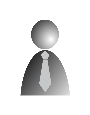
\includegraphics{./logos/decider-220x320.eps}};
  
% TOP DOWN linkings of the component IO structure:  
\draw[->,Gray] (Composer) to [out=270,in=90] (FRONTEND);
\draw[->,Gray] (FRONTEND) to [out=270,in=90] (FOUT);
\draw[->,Gray] (FOUT) to [out=270,in=90] (CONVERTER);
\draw[->,\mtexColor] (CONVERTER) to [out=270,in=90] (BIN);

\draw[->,\mtexColor] (BIN) to [out=270,in=90] (BACKEND);
\draw[->,Gray] (BACKEND) to [out=270,in=90] (PDF);

\end{tikzpicture}
\end{center}

Die verschiedenen Aufgaben solcher Systeme auseinanderzuhalten, ist bei der
Begutachtung von Lösungen essentiell. So attestiert z.B. eine ältere Sichtung
von Notensatzprogrammen der \enquote{Open Source Welt}, sie habe
\enquote{[\ldots] noch immer Schwierigkeiten, ein [\ldots] Nischenprodukt wie
ein Notensatzprogramm zu entwickeln}. Und sie begründet ihr Urteil damit, dass
\enquote{[\ldots] eine neue Mark-up-Sprache zu erlernen und in dieser grafische
Vorstellungskraft zu entwickeln [\ldots] nicht jedermanns Sache (sei)}, auch
wenn die Ergebnisse -- wie im Falle von \acc{Frescobaldi} und \acc{LilyPond} --
\enquote{[\ldots] äußerst professionell anmuten
(mögen)}.\footcite[vgl.][51]{Albrecht2009a} Wenn man, wie hier geschehen,
(graphische) Editoren und eigentliche Notensatzprogramme implizit 'gleichsetzt',
dann beraubt man sich der Möglichkeit zu einem differenzierteren und
pragmatischen Urteil: Wer integrierte Gesamtsysteme erwartet, bewertet komplexe
Architekturen mit verteilten Teilsystem eben dieser Verteilung wegen schlechter
-- und verkennt, das sehr viel komplexere Systeme nach diesem Prinzip aufgebaut
sind und erfolgreich betrieben werden, wie etwa \acc{Unix} resp.
\acc{GNU/Linux}.

Wir jedenfalls werden diesen Aspekten gesondert nachgehen: Zuerst analysieren
wir mögliche 'Backends' und deren Methoden, 'Noten' in \LaTeX-Texte einzubinden.
Sie sind insofern \acc{Backends}, als sie textuellen Input verarbeiten, der auch
über vorgelagerte, eher graphische Programme erzeugt werden könnte. Diese bilden
das 'Frontend' für den Arrangeur, Komponisten oder Musikwissenschafter. Solche
graphischen und semi-graphische Editoren und Konverter werden wir anlysieren,
nachdem die Backends begutachtet haben. Und ganz am Ende werden wir sehen, dass
uns gerade diese Aufteilung eine besondere Flexibilität bietet, Notenbeispiele
in (musik)wissenschaftliche Arbeiten einzubetten.

Allerdings werden wir uns bei unser Betrachtung auf die Open-Source-Welt
konzentrieren. Mehr oder minder konstenintensive proprietäre Programme mögen
beliebt sein, notwendig sind sie nicht. Es ist auch für den Musiker besser,
nicht in die 'Vendorenfalle' zu geraten und seine Arbeiten von den Produkten
einer Firma abhängig zu machen. Deshalb fokussieren wir uns hier auf die
Umsetzung mit freier Software.\footnote{Wer als Musiker proprietäre Programme
nutzt, macht sich erpressbar: Auf der einen Seite investiert er Zeit und Mühe in
die Erstellung von Notentexten, die er auch später noch weiterverarbeiten oder
wiederverwenden will. Auf der anderen Seite muss er fürchten, die hinter dem
eigenen Programm stehende Firma werde beim nächsten Versionswechsel die
Lizenzgebühren so stark erhöhen, dass sie das Budget des Musikwissenschaftlers
sprengen. Und selbst ohne diese finale Katastrophe wird der Wechsel zu einem
anderen Anbieter mit der Zeit durch die schon investierte Arbeit so aufwendig,
dass man lieber bei dem bisherigen Programm bleibt, auch wenn es teuerer oder
schlechter ist als die Alternativen. Damit ist man in die \textit{Vendorenfalle}
getappt. Mit freier Software kann das nicht geschehen, weil es zum Wesen freier
Software gehört, dass man ohne pekuniären Aufwand an den Quellcode und an die
Nutzungsrechte der ablauffähigen Programme herankommt - auch an die neuerer und
besserer Versionen. (\cite[vgl. dazu][\nopage wp.]{FSF2018a}.) Für Musiker hat
sich die Lage mit der Etablierung von \textit{MusicXML} allerdings etwas
entspannt: Durch die Standardisierung des Dateiformates wird der Wechsel zu
einem anderen, besseren Programme erleichtert. Hier muss man 'nur' noch
fürchten, dass das bisher die jeweiligen Programme vorab (noch) nicht
standardisierte Features benutzen oder den Standard nicht ganz konform
implementiert haben. Allerdings sind solche 'Eigenarten' ein beliebtes Mittel,
den zahlenden Kunden zuletzt doch wieder an sich zu binden und ihm den Wechsel
zur Alternative zu erschweren. (\cite[Zur Lizenzierung von MusicXML vgl.
auch][\nopage wp.]{WpedMusicXML2018a}) Dieser Kontext gibt uns auch die
Gelegenheit, auf die Lizenzproblematik einzugehen: Wir werden bei den Tools
jeweils kurz nachweisen, dass es es sich tatsächlich um freie Software bzw. Open
Source Software handelt. Dass dem so ist, ist uns wichtig. Denn aus einem
solchen Nachweis ergibt sich, dass man die Software ohne Einschränkungen und
unentgeltlich nutzen darf. Allerdings folgt Open Source Software dem Prinzip
'Paying by Doing'. Anstatt -- wie sonst üblich -- die Nutzungsrechte zu kaufen,
'erwirbt' man diese, indem man das aktiv tut, was die Lizenzen dem Nutzer
auftragen. Zu wissen, was das ist, ist kein Hexenwerk, kann in Einzelfällen aber
'tricky' werden. Diese rechtlichen Rahmenbedingungen sind nicht unser Thema. Wir
gehen deshalb davon aus, dass Sie sich selbst darum kümmern werden, wenn es
angesagt ist. Unser Erfahrung nach gibt es dafür eine gute Daumenregel: Sie
dürfen die Frage, ob und wie sie die Software lizenzkonformen nutzen, solange
aufschieben, bis Sie sich entscheiden, die Software an andere weiterzugeben.
Oder anders gesagt: Solange Sie selbst diese Software 'nur' von irgendwoher
downgeloaded oder installiert haben und anwenden, solange dürfen Sie die
Beachtung der Compliance auch 'recht gefahrlos' auf später verschieben.}

Dazu noch einige abgrenzende Worte:
\begin{itemize}
  \item Damit Sie einen guten Gewinn von der Lektüre haben, sollten Sie mit der
  Nutzung von \LaTeX\ unter Ihrem Betriebssystem vertraut sein.
  Insbesondere die Erweiterung Ihres \TeX-Systems und die Installation von
  zusätzlichen CTAN-Paketen legen wir kommentarlos in Ihre Hände\footnote{Es
  gibt eine Fülle guter, auch auf die Praxis ausgerichteter \LaTeX-Einführungen.
  (\cite[etwa][7ff]{Schlosser2016a}). Die ma\-nuelle Installation eines
  CTAN-Paketes ist -- wenn überhaupt nötig -- so schwierig nicht: Man lädt sich das
  Paket herunter und entpackt es in einem Ordner. Dann kopiert man diesen Ordner
  -- nötigtenfalls mit Root-Rechten -- in die \LaTeX-Distribution, z.B. unter
  \texttt{/usr/share/texmf/tex/latex/} (wobei \acc{/usr/share/texmf}
  distributionsabhängig ist). Und schließlich setzt man an der Konsole / im
  Terminal noch einmal das Kommando \texttt{sudo texhash} ab, um das neue Paket
  bekannt zu machen. Wenn Sie eine gängige Distribution benutzen, sollte der
  Rückgriff auf solch eine Detailarbeit aber gar nicht nötig sein.}.
  \item Ferner setzen wir voraus, dass Sie die Tools und Programme, die wir
  erwähnen, unter Ihrem Betriebssystem installieren können.
  \item Außerdem werden wir Sie nicht anleiten, wie man mit einem der
  begutachteten System Notentexte schreibt. Dazu gibt es bessere und genauere
  Handbücher, auf die wir gerne und dankbar verweisen. Was wir Ihnen jedoch
  zeigen werden, ist, wie man die mit den Tools erarbeitete Notentexte - wenn
  überhaupt möglich - in einen \LaTeX-basierten wissenschaftlichen Text
  integriert.
  \item Und schließlich gehen wir ohne große Prüfung davon aus, dass die
  Programme und Tools, die behaupten, für verschiedene Betriebssysteme zu
  existieren, im wesentlichen gleich funktionieren. In der Open-Source-Welt ist
  dem üblicherweise so.
\end{itemize}

Und damit wollen wir es gut sein lassen mit dem Erwartungsmanagement.



% this is only inserted to eject fault messages in texlipse
%\bibliography{../bib/literature}
